\section{Evaluation}~\label{sec:evaluation}

In this section, we empirically evaluate our techniques against other \pr clause
learning techniques. In doing so, we aim to answer the following research questions:


\begin{enumerate}
    \item Can our approach provide short \pr proofs for certain benchmark families?
    \item Is our approach less sensitive to encoding choices compared to other
    \pr learning techniques?
    % \item Can these techniques underperform or outperform SAT solvers on other certain benchmark
    % families?
\end{enumerate}

% We do so by implementing our technique in a tool \tool (a fork of \cadical
% commit f13d74439a5b5c963ac5b02d05ce93a8098018b8). 

The two main techniques for learning \pr clauses are \sadical (based on SDCL)
and \prelearn (a preprocessing techniques that calls \sadical). We also compare 
to \cadical, as a baseline with no \pr clause learning.

In \autoref{subsec:eval-pigeonhole}, we compare \tool to \cadical and \sadical
on the pigeonhole principle. We evaluate based on time taken, the length of
the proof, and the sensitivity to the encoding of the formula. 

% In \autoref{subsec:eval-chess}, we compare augment \tool with fixed
% heuristics to discover $O(n^3)$ proofs of mutilated chessboard. We compare to the best known
% mutilated chessboard \pr proof~\cite{mutilatedchessboard-pr}.

In \autoref{subsec:eval-satcomp}, we evaluate the solvers on benchmarks from the
annual '22, '23, and '24 SAT competition's main
tracks~\cite{satcomp2022,satcomp2023,satcomp2024}.

In \autoref{subsec:eval-discussion}, we highlight certain benchmark families
that benefit from and are hurt by \pr clause learning. We evaluate the different approaches on these families.


Finally,we analyze the use of specific heuristic choices in \tool
by turning heuristics off one by one and observing the effect on the performance
on those benchmarks families (\autoref{subsec:eval-heuristics}). 

All experiments were performed in the Anvil Supercomputing Center on nodes with
128 cores and 2 GB RAM~\cite{anvil}. We ran 64 experiments in parallel per node
with 5,000 second timeouts.

\subsection{Pigeonhole results}~\label{subsec:eval-pigeonhole}

We compare the performance of \tool, \cadical, \sadical, and \prelearn on
pigeonhole principle benchmarks up to size $40$. Approaches based on SDCL, such
as \sadical, were successful at learning short proofs for the pigeonhole
principle, but were very sensitive to how the problem was encoded.

As shown in \autoref{fig:pigeonhole-results}, \prelearn, \sadical, and \tool scale cubicly
in both runtime and proof size. Interestingly, \tool is able to learn shorter
proofs by a factor of $2$-$5$x compared to \prelearn. As we discuss in
\autoref{app:pigeonhole}, \tool learns proofs of size $\approx \frac13 n^3$,
which is expected to be shorter than known \pr proofs for the pigeonhole principle.

Additionally, we evaluate all solvers on scranfilized variations of the
pigeonhole principle. Scranfilization is a technique for generating an
equivalently satisfiable formula from an existing one by permuting variables,
permuting clauses, and flipping literals~\cite{scranfilize}. We use the tool
\texttt{scranfilize} with configurations permuting variables,
and permuting clauses turned on, and flipping literals turned on with
probability $0.5$~\cite{scranfilize}. We run each solver on 5 scranfilized variations for
each benchmark and take the median runtime and proof size. This is shown in \autoref{fig:pigeonhole-results} with dashed lines.


Both \sadical and \cadical exhibit an exponential trend when run on the scranfilized benchmarks for runtime and proof size. However, \tool can almost match its non-scranfilized performance, demonstrating that it learns useful \pr clauses regardless of the encoding of the formula.

In conclusion, \tool is able to match \sadical's runtime for the pigeonhole principle while shorter proofs by a constant factor. Additionally, \tool is insensitive to permuting variables, permuting clauses, and flipping literals as it relies on conditional autarkies, a global property of the formula.


\begin{figure*}[!t]
    \centering
    \begin{subfigure}[t]{0.4\textwidth}
        \centering
        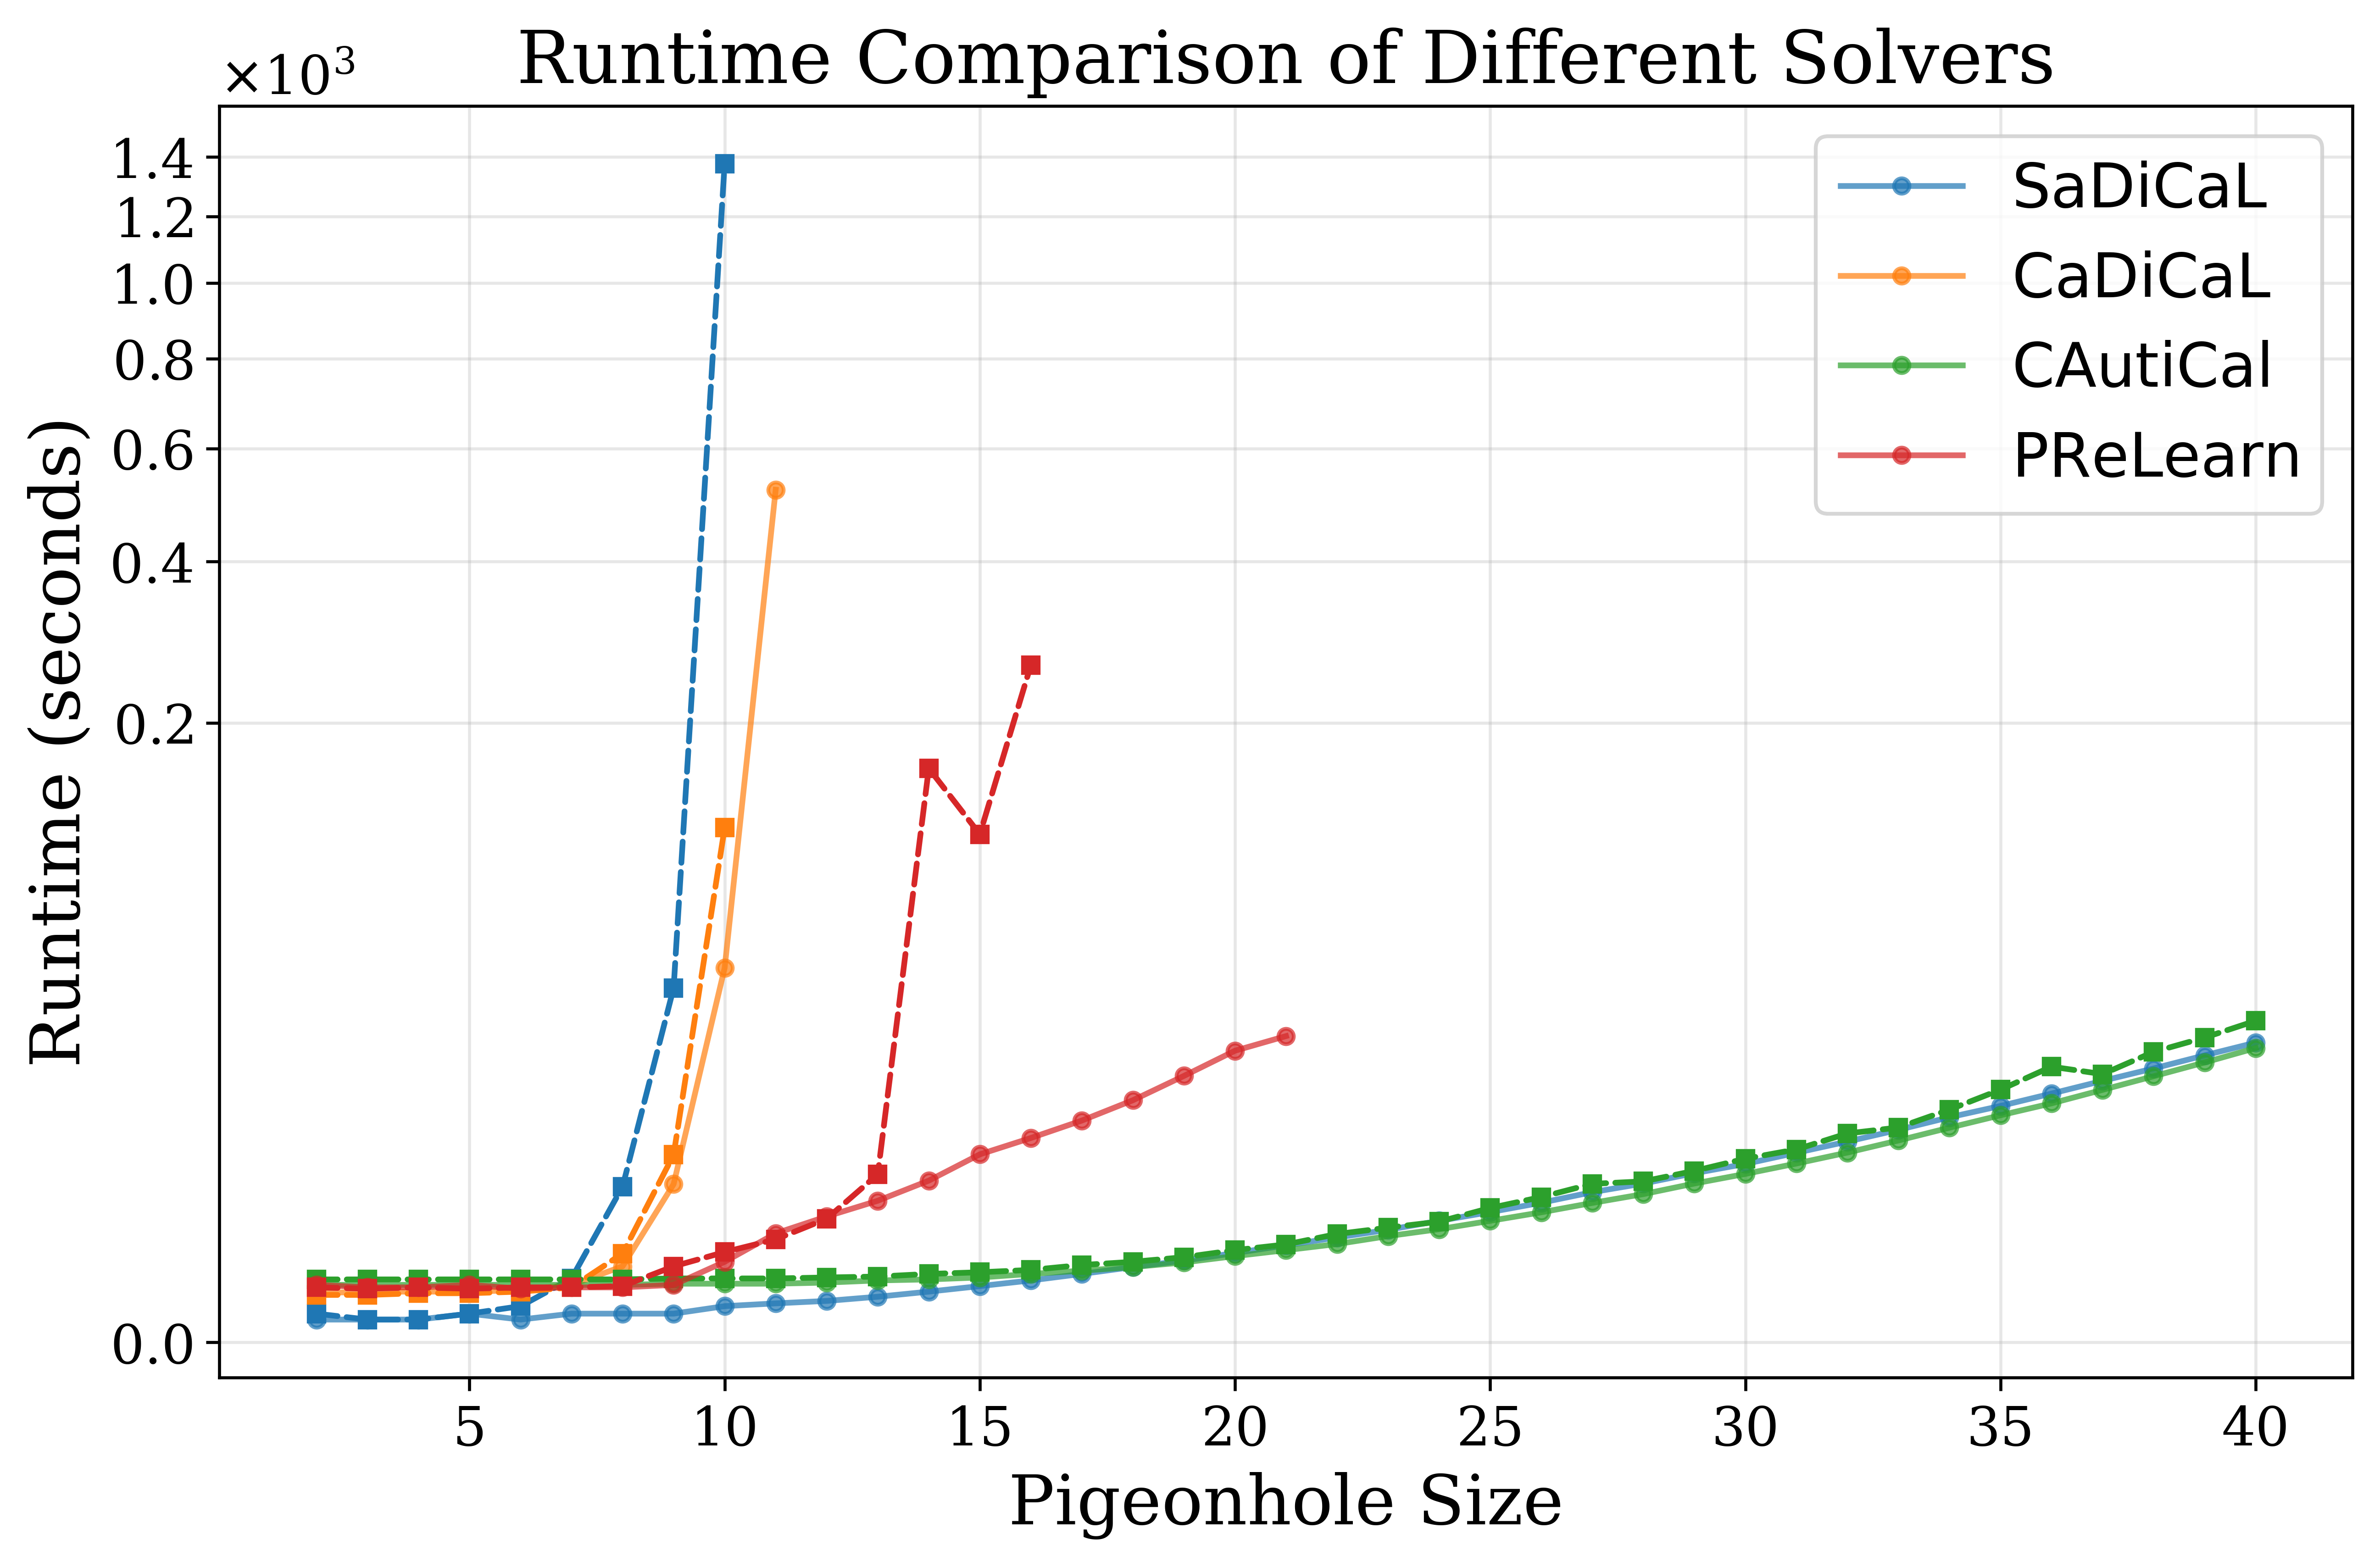
\includegraphics[width=\textwidth]{figs/pigeonhole_runtime_comparison.png}
        \caption{Runtime on Pigeonhole Principle Formulas}
        \label{fig:pigeonhole-runtime-comparison}
    \end{subfigure}
    \hspace{0.06\textwidth}
    \begin{subfigure}[t]{0.4\textwidth}
        \centering
        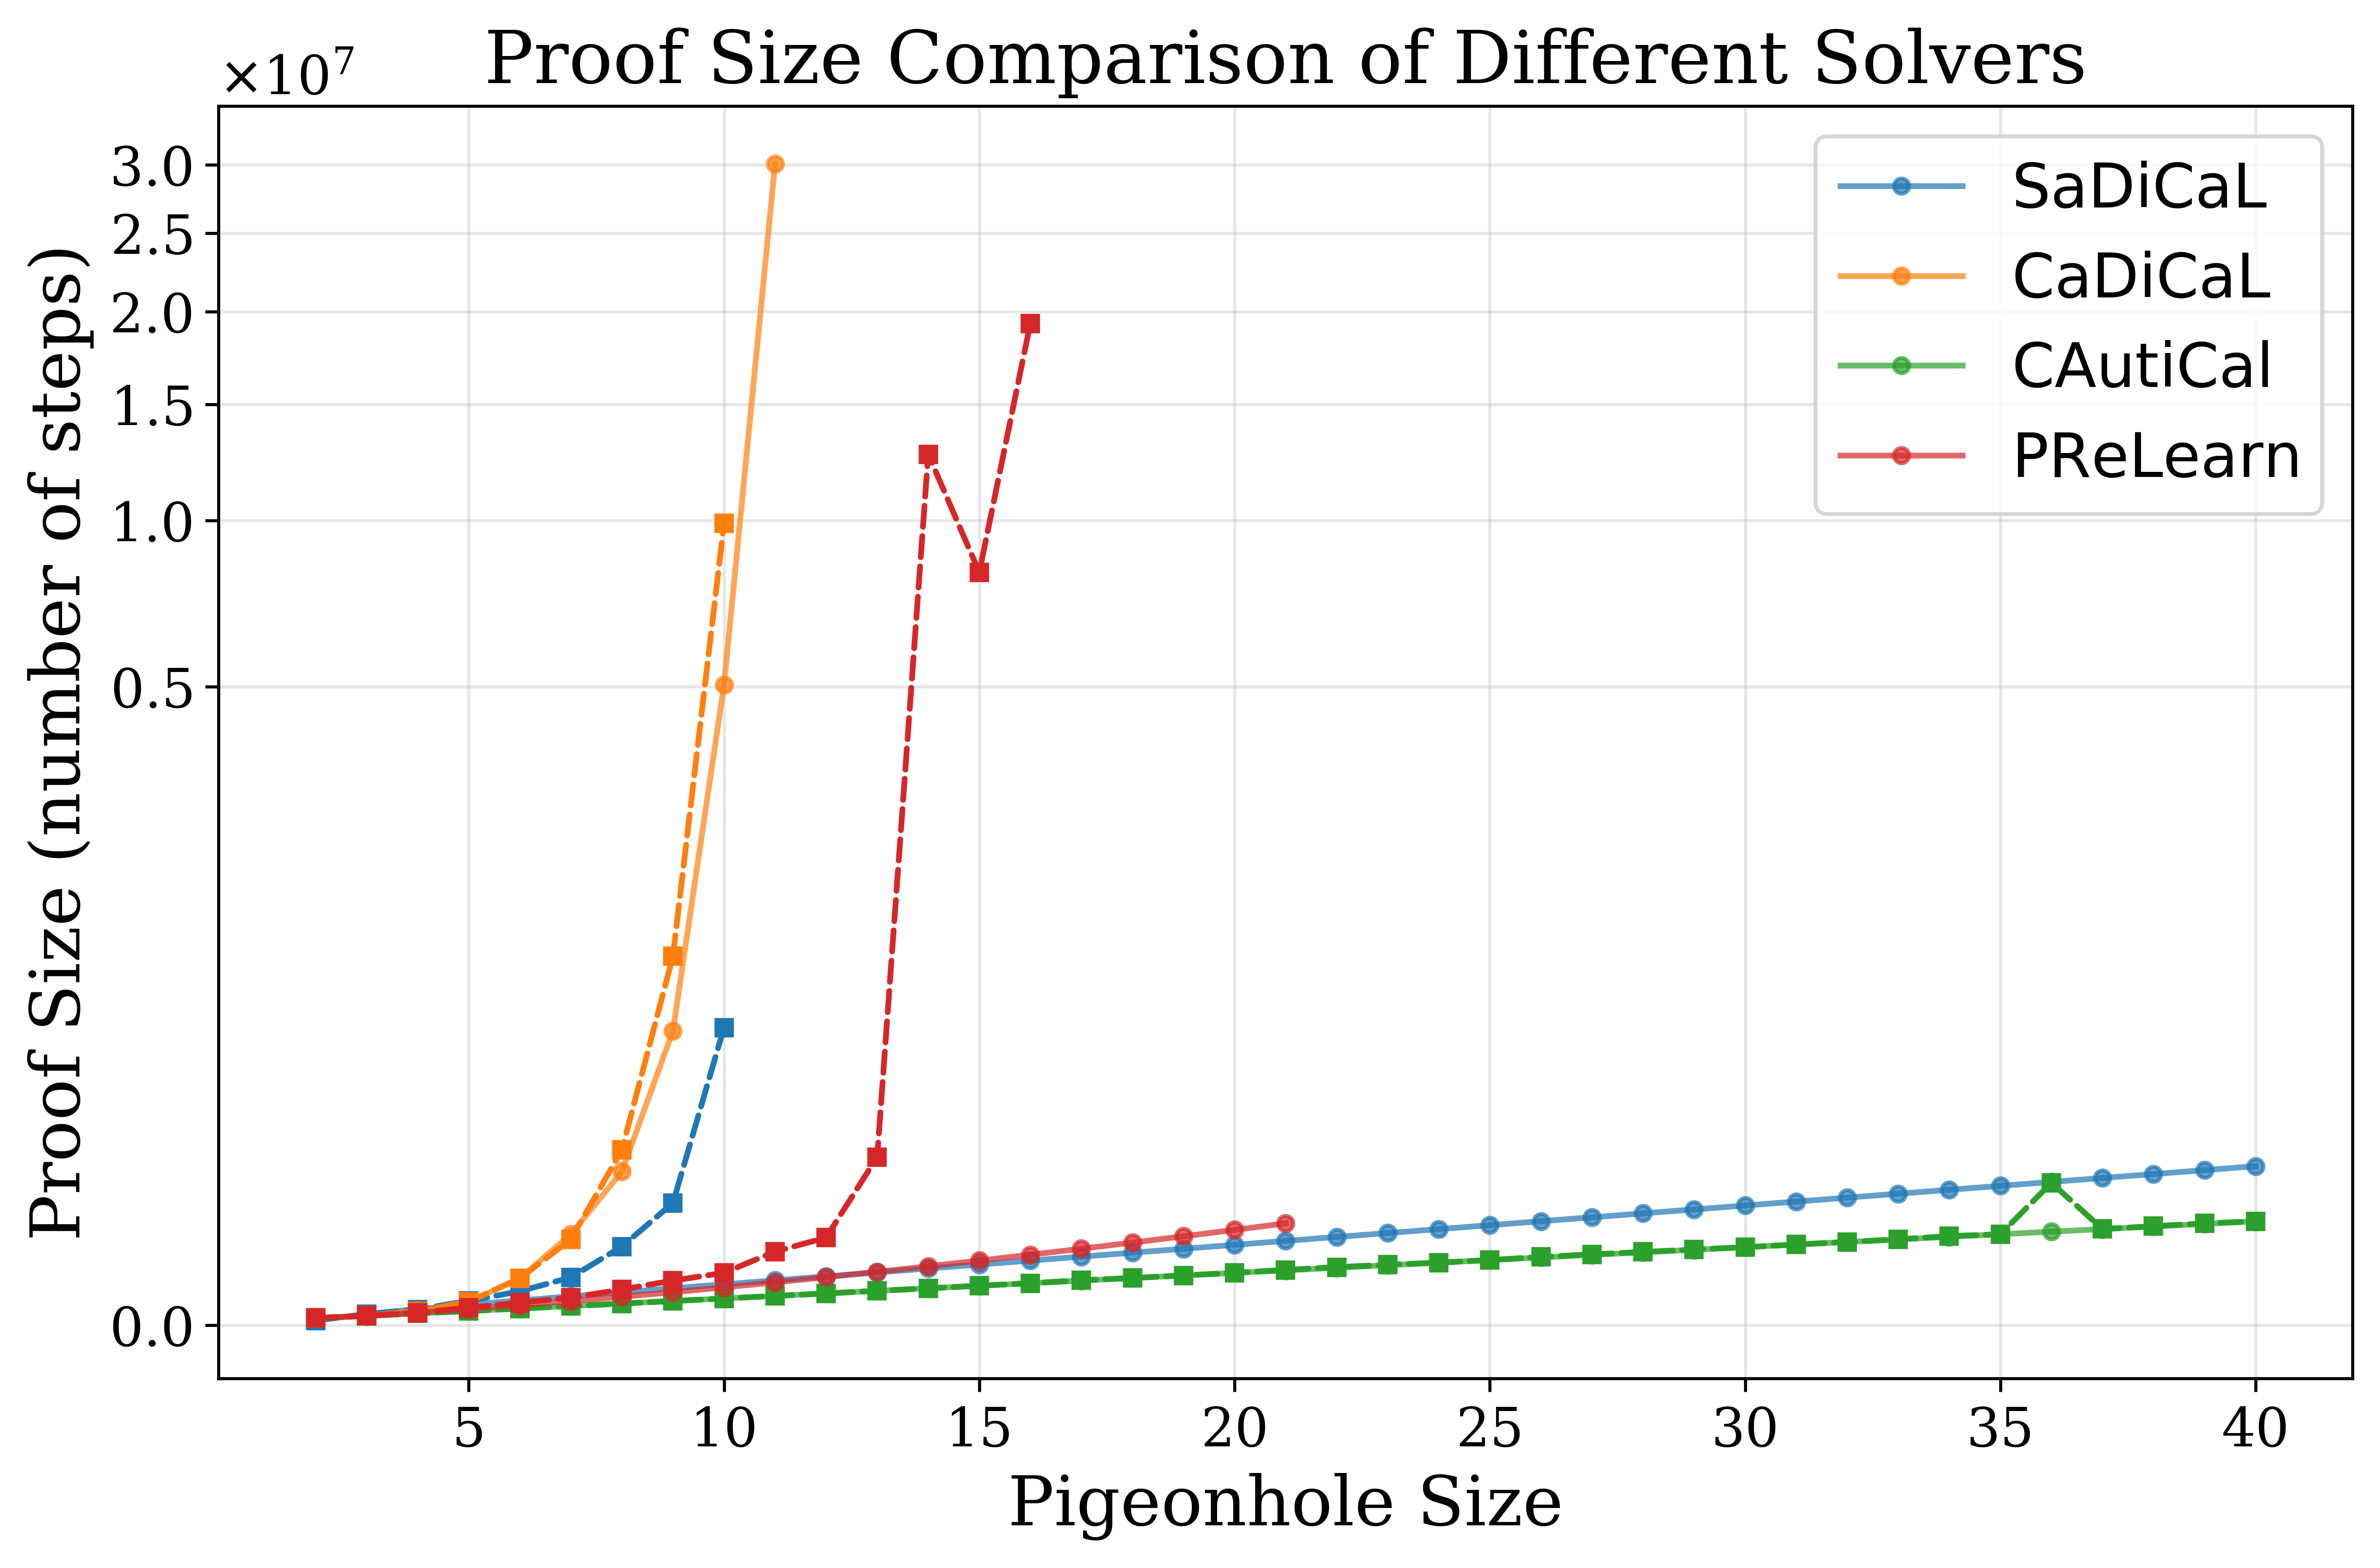
\includegraphics[width=\textwidth]{figs/pigeonhole_proof_size_comparison.png}
        \caption{Proof Size for Pigeonhole Principle Formulas}
        \label{fig:pigeonhole-proof-size-comparison}
    \end{subfigure}
    \caption{Comparison of \tool, \cadical, \sadical, and \prelearn on pigeonhole principle benchmarks up to size $40$. The y-axis is on a cube root scale. The performance of a solver on the original benchmark is shown with a solid line. The median of 5 scranfilized queries is shown with a dashed line. If a solver times out on a query in 5000s, it is not shown.}
    \label{fig:pigeonhole-results}
\end{figure*}

% \subsection{Mutilated chessboard results}~\label{subsec:eval-chess}


\subsection{SATCOMP results}~\label{subsec:eval-satcomp}

\begin{figure*}[!t]
    \centering
    \begin{subfigure}[t]{0.4\textwidth}
        \centering
        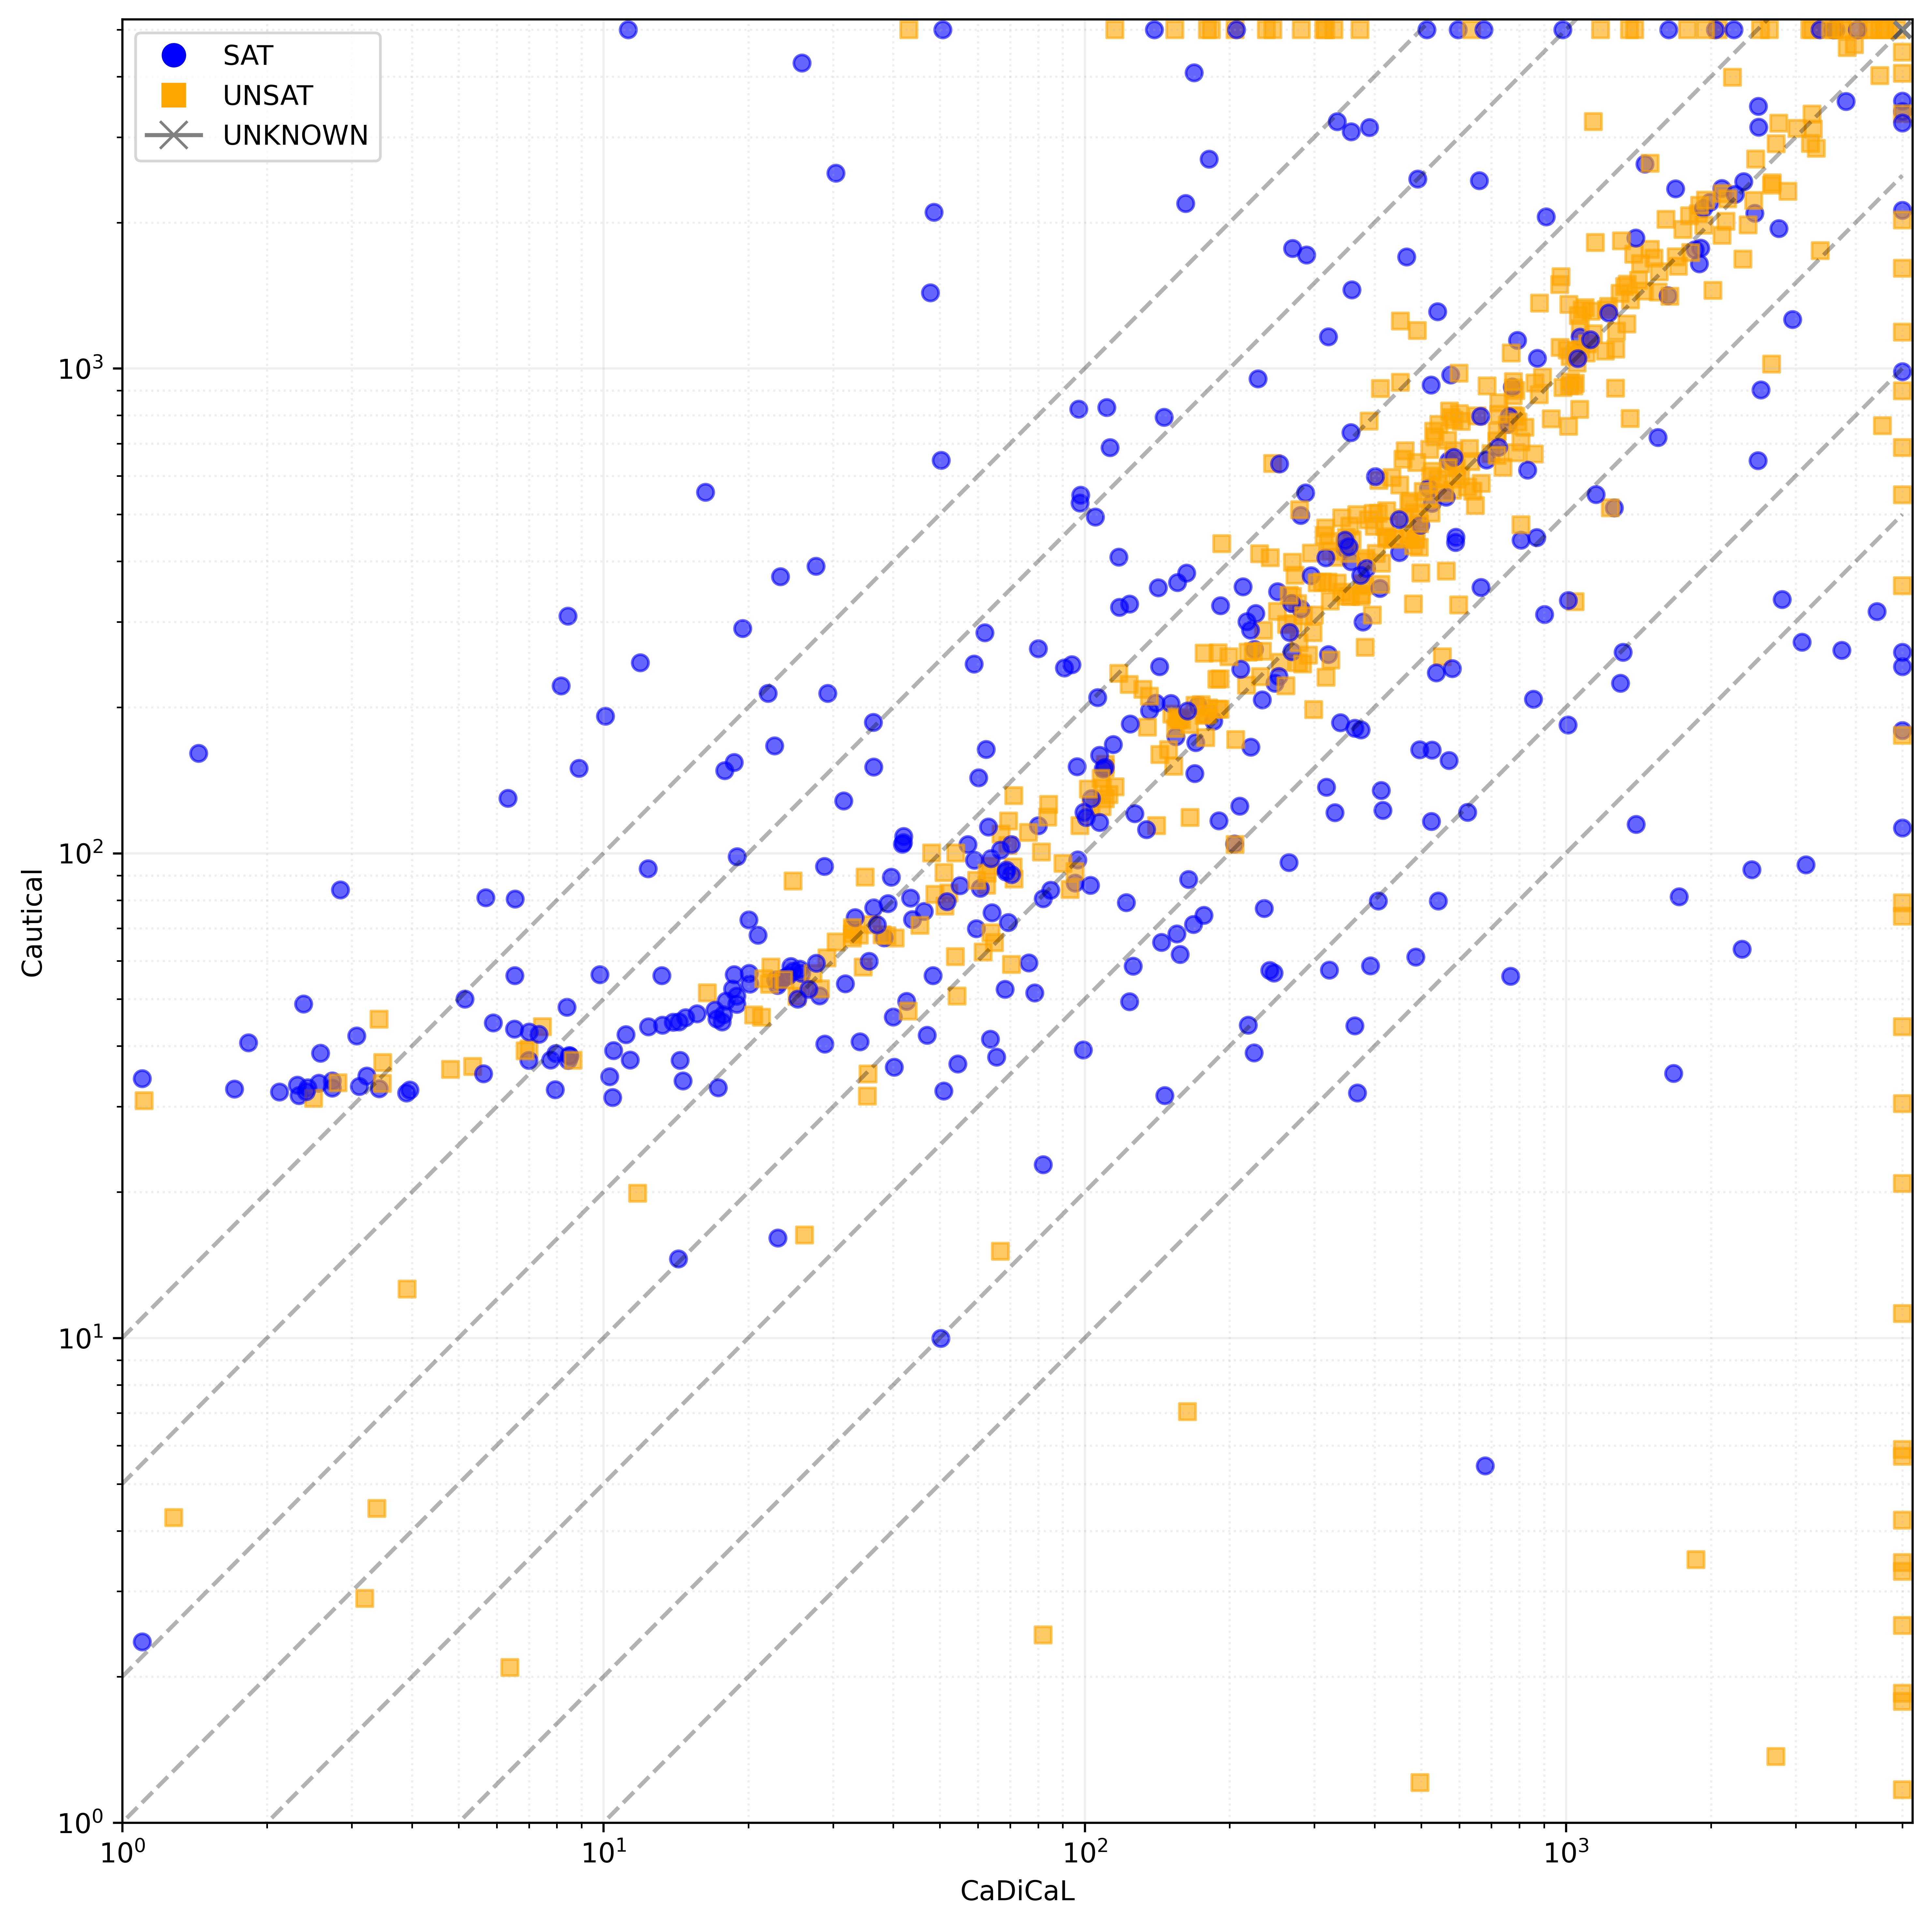
\includegraphics[width=\textwidth]{figs/cautical_vs_cadical_log.png}
        \caption{Comparison with \cadical}
        \label{fig:cautical-vs-cadical}
    \end{subfigure}
    \hspace{0.06\textwidth}
    \begin{subfigure}[t]{0.4\textwidth}
        \centering
        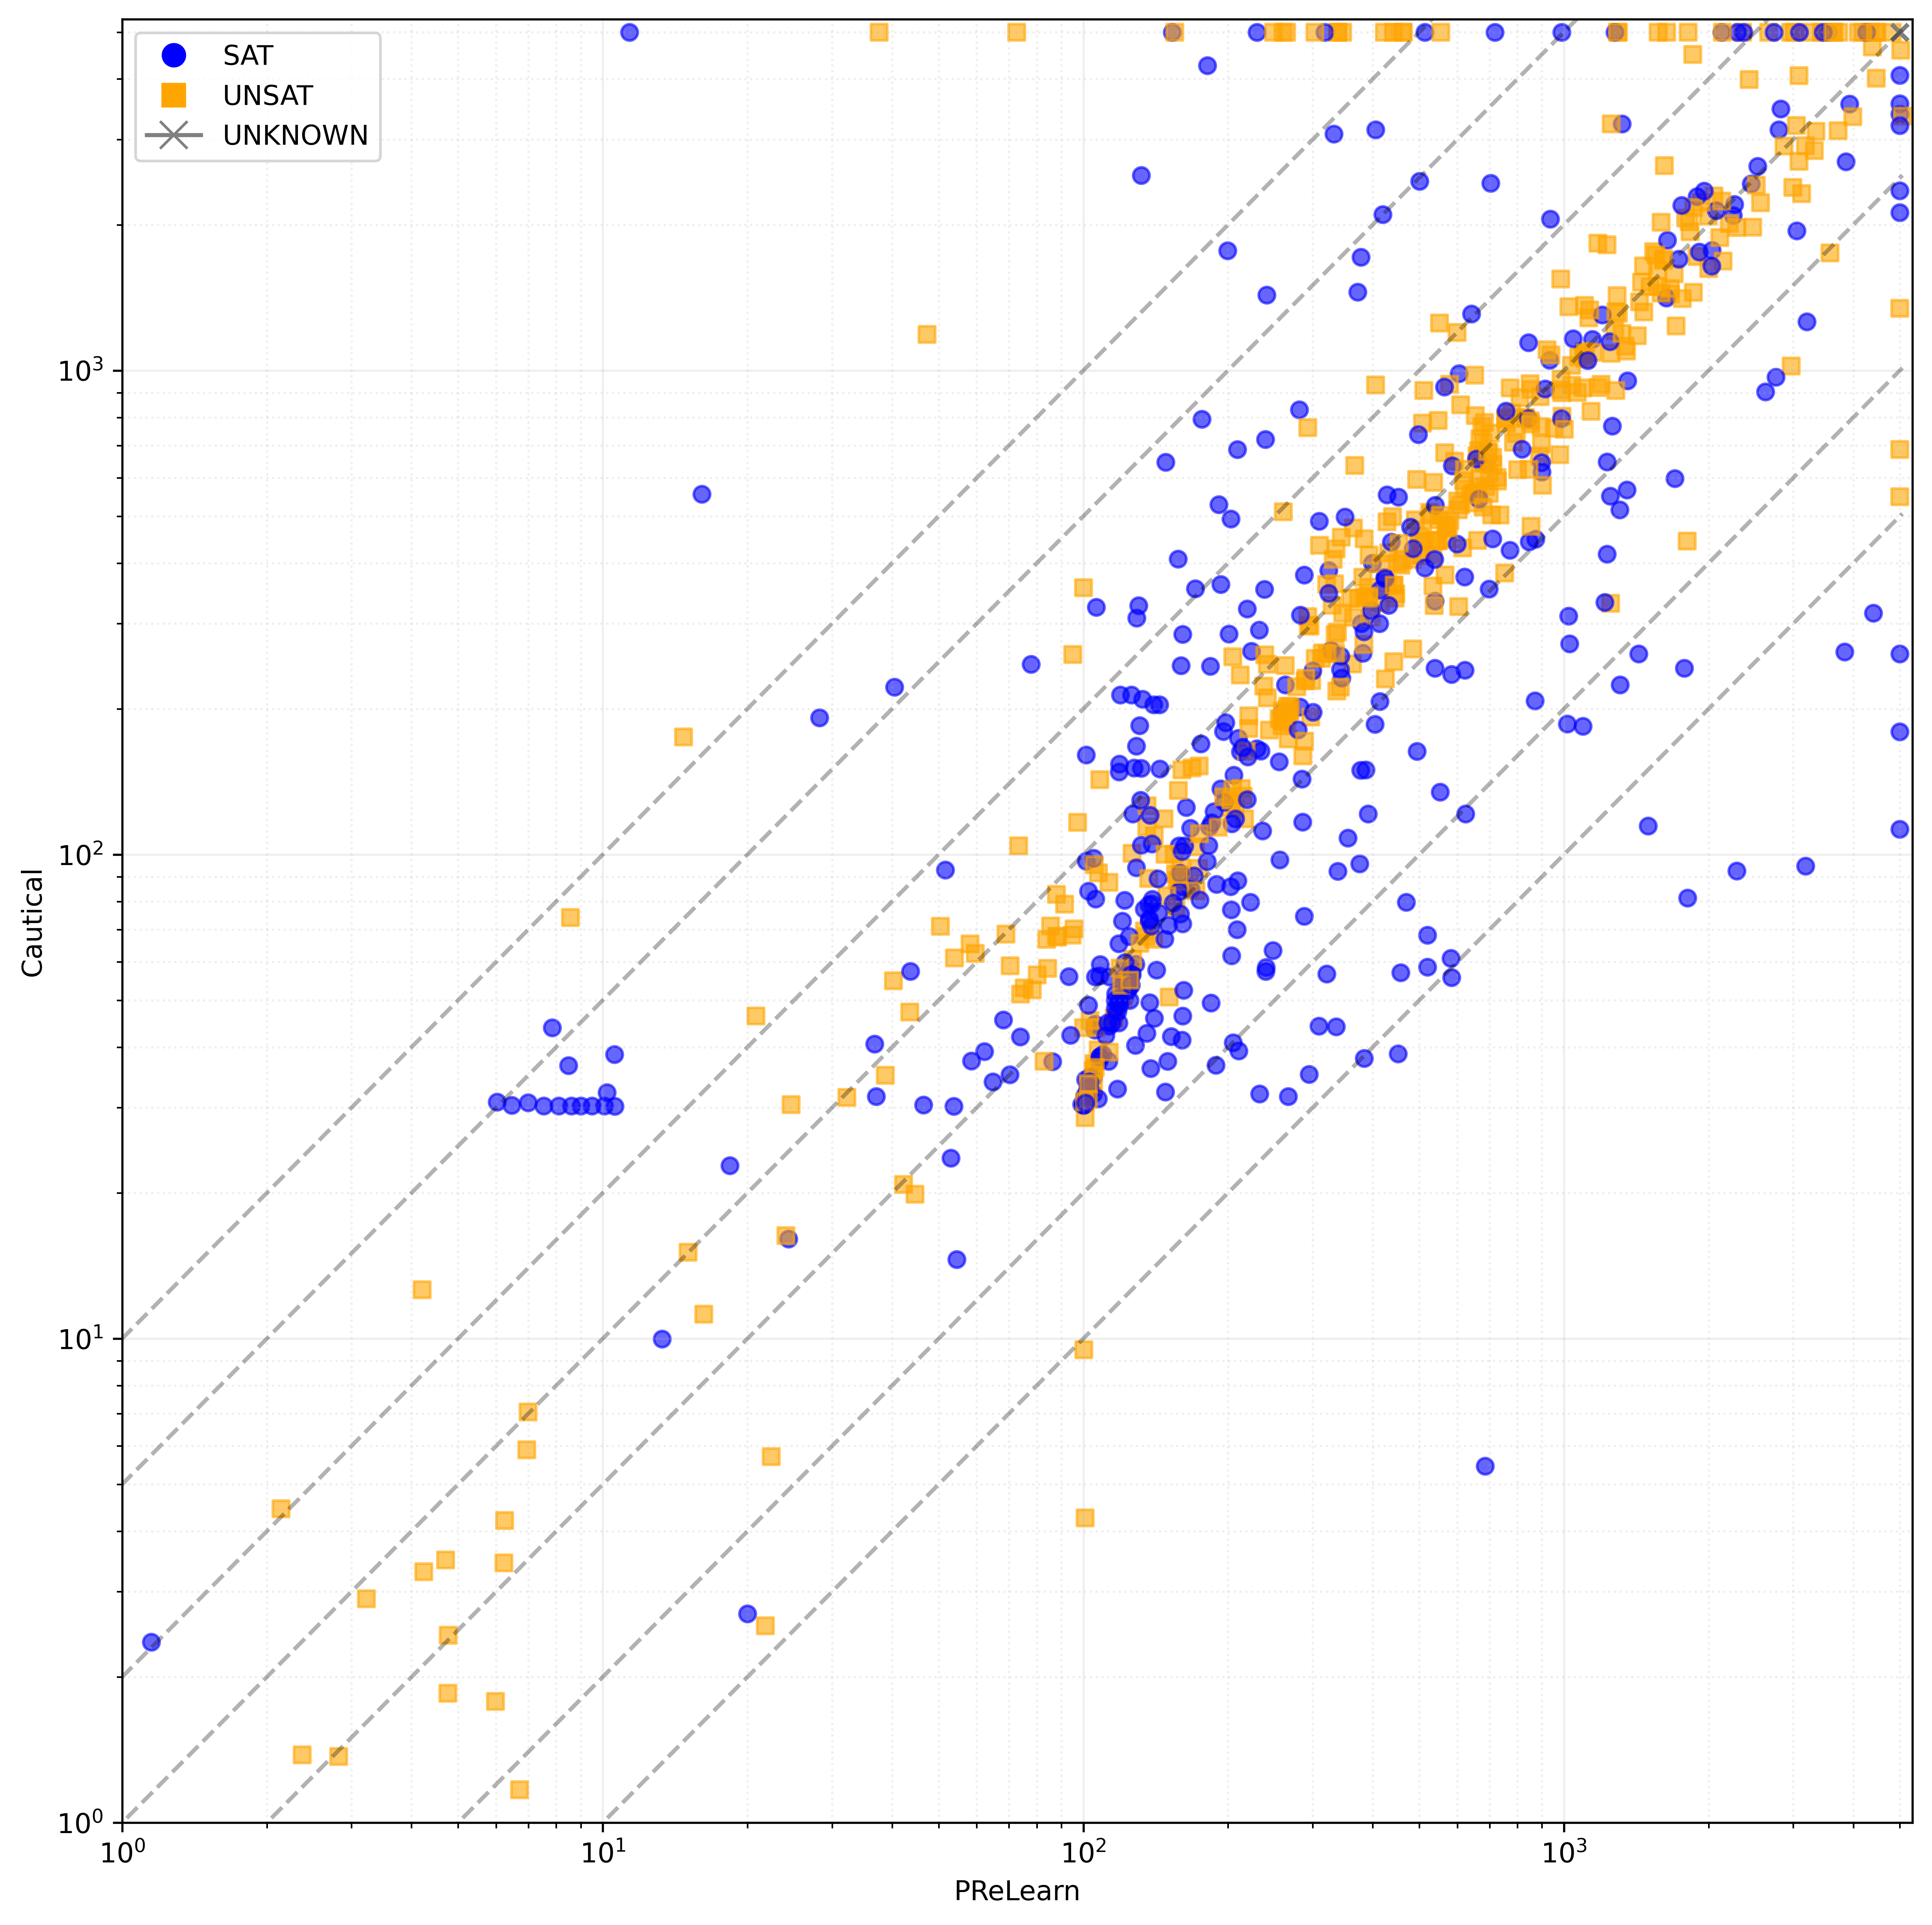
\includegraphics[width=\textwidth]{figs/cautical_vs_prelearn_log.png}
        \caption{Comparison with \prelearn}
        \label{fig:cautical-vs-prelearn}
    \end{subfigure}
    \caption{Performance comparison of \tool with other solvers}
    \label{fig:solver-comparison}
\end{figure*}

In \autoref{fig:solver-comparison}, we compare the performance of \tool with \cadical and \prelearn on the benchmarks from the annual Satisfiability competition from the years 2022, 2023, and 2024. \autoref{tab:solver-stats} shows the number of instances solved by each solver as well as the number of queries for which \prelearn and \cadical learn additional clauses, improve upon \cadical, and solve that \cadical does not solve.

The PAR-2 score is used to evaluate the performance of the solvers at the competition, it is the sum of the runtime on instances solved plus two times the timeout for each instance unsolved. On this dataset, \cadical has a PAR-score of 3970200.7 seconds, \prelearn has a PAR-score of 3791297.9 seconds, and \tool has a PAR-score of 4072090.4 seconds.

\begin{table}[ht]
    \centering
    \sisetup{table-format=3}        % remove if you are not using siunitx
    \begin{tabular}{lrrrr}
      \toprule
      & \multicolumn{2}{c}{0--10k} & \multicolumn{2}{c}{10k$+$} \\
      \cmidrule(lr){2-3} \cmidrule(lr){4-5}
      & SAT & UNSAT & SAT & UNSAT \\
      \midrule
      \cadical Solved      &  54 &  73 & 354 & 349 \\
      \midrule
      Total w/ \prelearn &  52 &  92 & 356 & 355 \\
      \prelearn learnt      &  43 &  75 & 216 & 203 \\
      Improved w/ \prelearn&  12 &  31 &  32 &  22 \\
      Only w/ \prelearn    &   1 &  19 &   6 &   9 \\
      \midrule
      Solved w/ \tool  &  52 &  87 & 349 & 327 \\
      \tool learnt     &  16 &  59 &  32 &  36 \\
      Improved w/ \tool&  23 &  33 &  87 &  78 \\
      Only w/ \tool    &   0 &  18 &   9 &   9 \\
      \bottomrule
    \end{tabular}
    \caption{Number of solved instances.}
    \label{tab:solver-stats}
  \end{table}

  

% \subsection{Analysis of heuristics}~\label{subsec:eval-heuristics}

% \subsection{Discussion of Benchmark Families}~\label{subsec:eval-discussion}